\section{Challenges with the search method and tools}

In the previous sections, the output and results of using the autoencoder for anomaly detection have been shown. 
The method and results, as produced and shown in this thesis, have yielded some promising results given the nature 
of the search method. However, it should be known what the challenges of the task actually are to truly understand 
why the results are only promising, and not great compared to other search methods. The challenges can be divided into 
three main points, all of which are entangled together. The three challenges are listed below. 

\begin{itemize}
    \item Model independence
    \item Reconstruction error minimization
    \item Feature engineering
\end{itemize}

Model independence is the first challenge. By model, it is here referring to signal models. 

As mentioned in the theory section for the SM, 
the SM, although very successful in certain predictions, lack the ability to explain a whole number of 
behavior around us, and so there have been made many suggested solutions to the issues. These new models are 
often called extensions to the SM, and although mathematically consistent, not neccesarly physically possible. 
And even if they are physically possible, in other words, they adhere to certain fundamental physical principles, they 
still might not exist, as several searches at ATLAS have excluded but never found any new physics. 

The search method is inherently 
biased as one assumes that the new physics looks like the signal, and thus do analysis, data preparation etc. with that 
signal in mind. But we do not know, at all, what the new physics looks like, even the assumption that we are looking for 
particles are implying a bias that might not be true. From the collisions in the detector to the analysis, there are biased descisions, 
we cannot avoid them, but we can minimize them as much as possible, which is a goal with the search strategy in this thesis. \par

This leads us to the second challenge, which is reconstruction error minimization. The proposed method in this thesis is to 
learn the signature of the SM so well, that even subtle anomalous behavior will be picked up by the analysis tool. 
The autoencoder learns the signature of the SM via reconstruction error minimization, and then hopefully the 
anomalous data will be picked up in a signal region. One problem with this is that one first blinds oneself to signals 
that might be very, very similar to the SM in some feature space, but with very low statistics. These events 
will for a given set of features, never be found. \par 

The third challenge is the choice of features. This thesis utilized the RMM structure by Chekanov et al., as it maximizes 
the amount of information in the input data by using almost completely uncorrelated features. However, as we do not know the signals 
we are looking for, there is no way to know if this choice is the optimal choice for new physics. In fact, even if we found 
an ideal set of features, based on some physical principles or something else, it is not trivial that the reconstruction error calculation
should weight the error of each feature equally. It might very well be that some features are less important than others. Essentially, 
the goal is to optimize for a signal we do not know, using features we don't know are optimal, and weighting them as "unbiased" as 
possible, simply taking the average, to dictate how the autoencoder learns and updates its internal weights and biases. 

\section{Future work}

Autoencoders and their applications to anomaly detection in high energy physics are not well understood, 
and this thesis on scraped on some issues and attempts that needs to be done. It is a recent topic in within 
the HEP community, and consequently much work is needed to reach a better understanding of how autoencoders 
behave with HEP data. The work done in this thesis has led to three areas of focus that should be explored more, 
listed below. 

\begin{itemize}
    \item Computational bottlenecks 
    \item Data and feature engineering 
    \item Network and architecture engineering
\end{itemize}

\subsection*{Computational bottlenecks}
From sections \ref{sec:3lep} and \ref{sec:2lep} there seems to be a positive trend in increasing the amount 
of training data for the autoencoders, both regular and variational. With a continual increase in data from 
Run3 and onward \cite{LHC_int_lum}, so will the loading and storing time used for doing analyses increase. 

\begin{figure}[H]
    \caption[LHC nominal luminosity projections]{LHC nominal luminosity projections for the next 2 decades}
    \label{fig:lhc_nom}
    \centering
    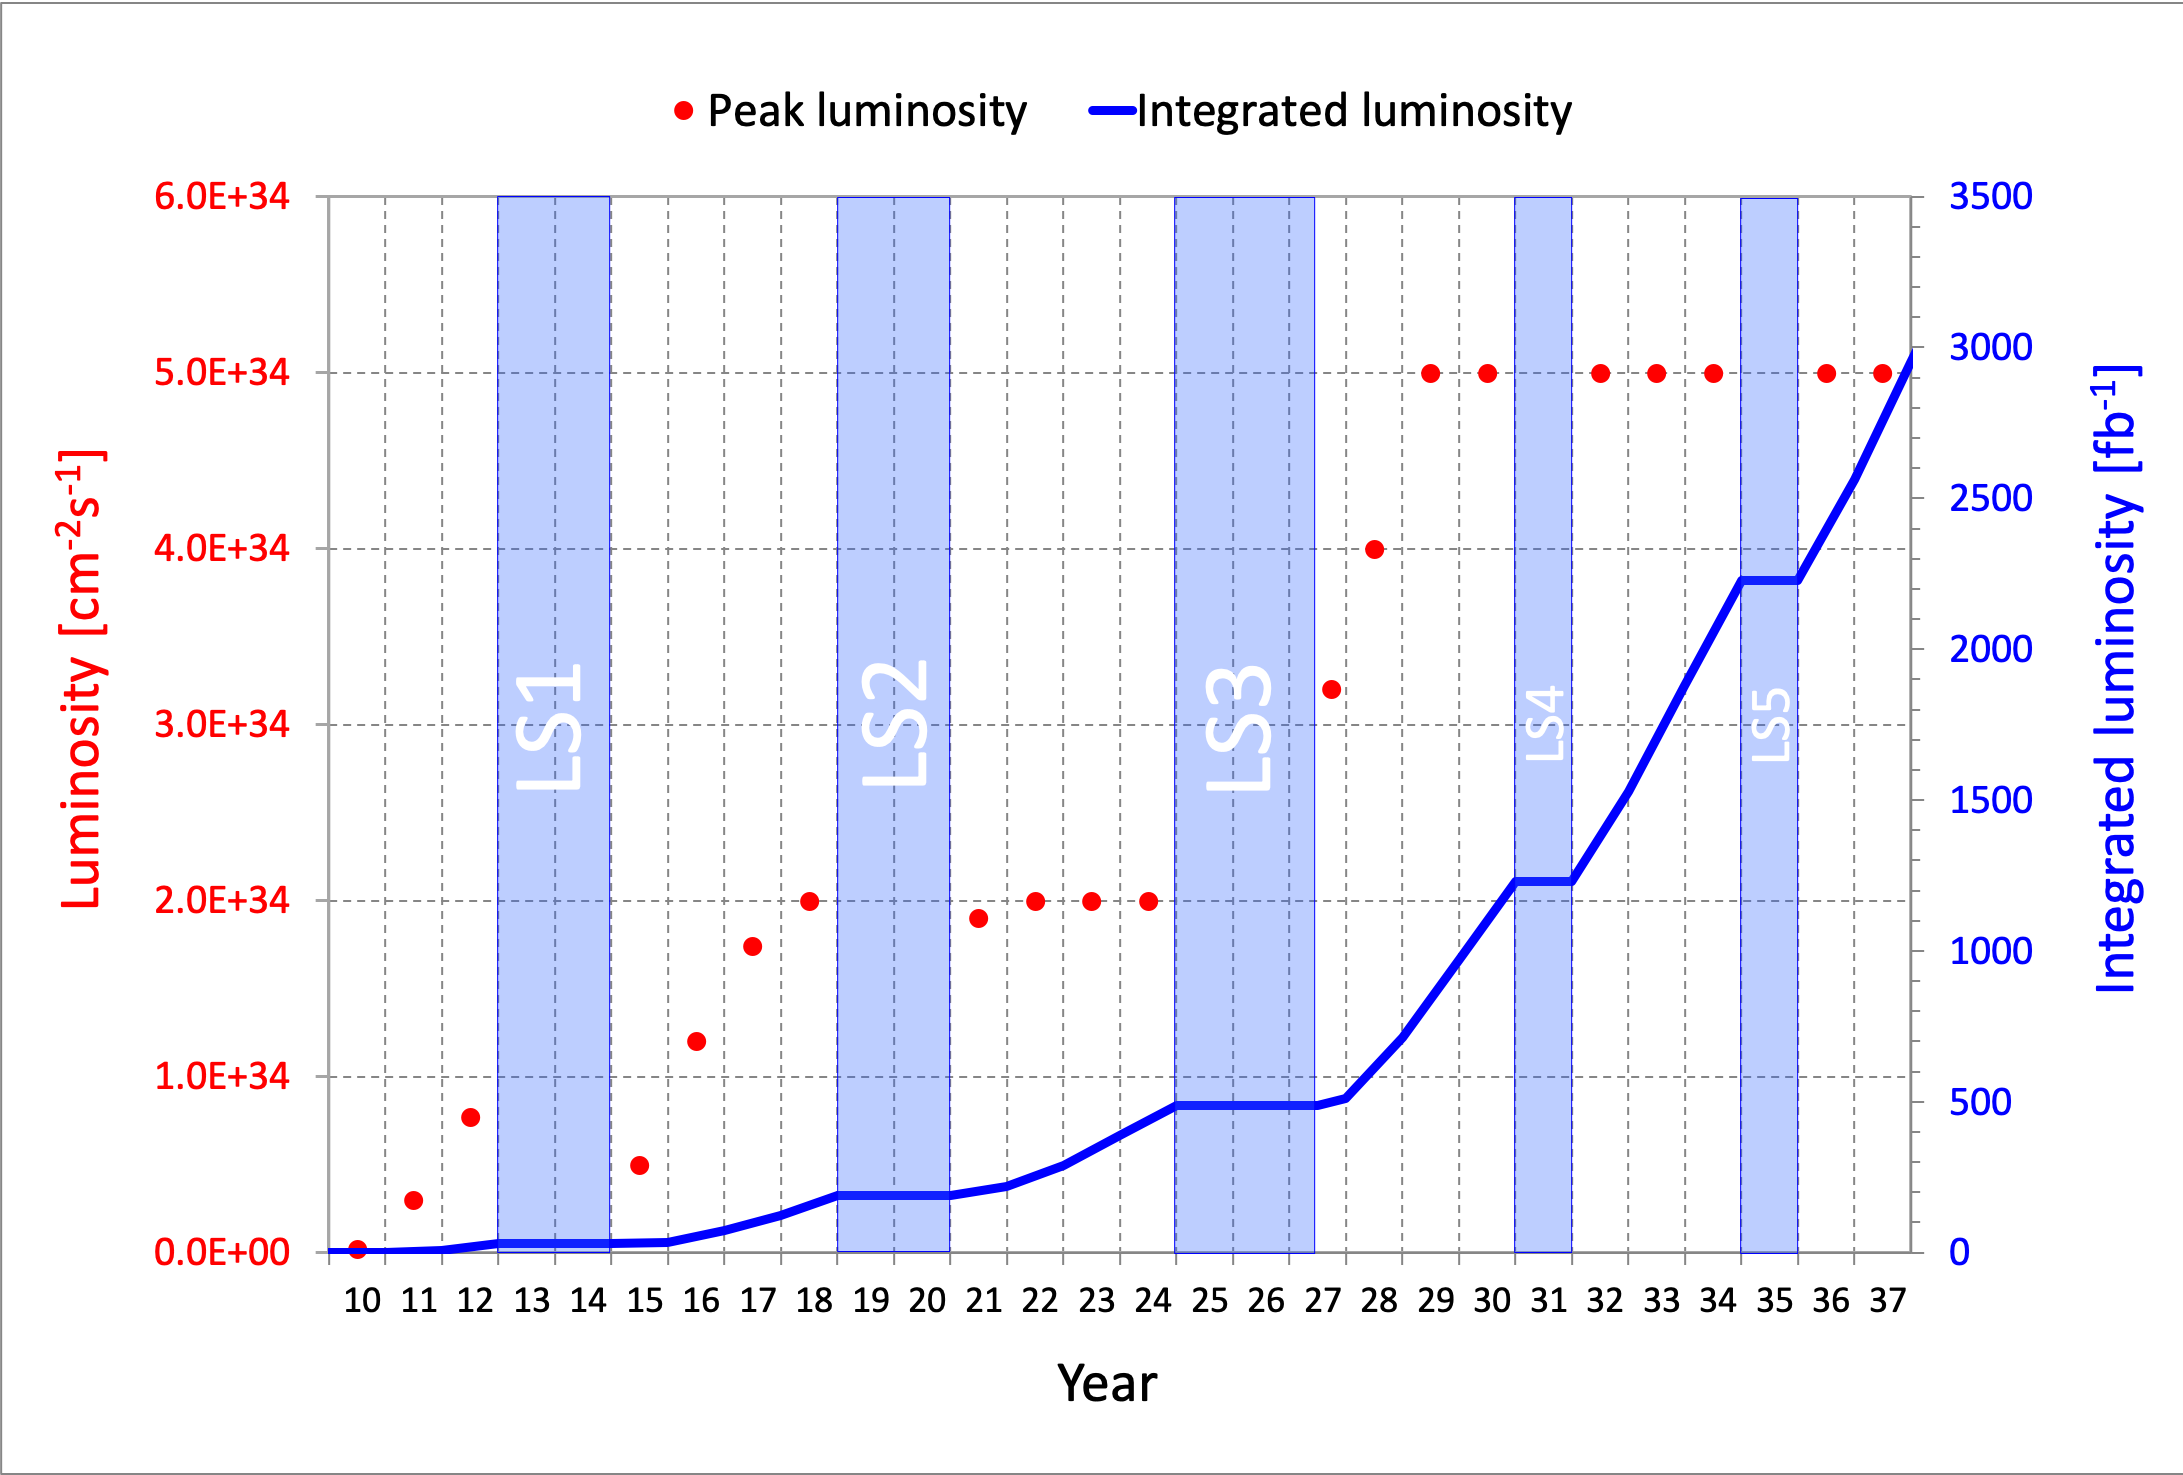
\includegraphics[width=0.7\textwidth]{Figures/atlas/LHC-nominal-lumi-projection.png}
\end{figure}
Figure \ref{fig:lhc_nom} shows the expected time periods for data collection and the amount of data expected for 
the next two decades. \par
One bottleneck\footnote{The bottleneck problem explained here is not in regard to the recording of the events. 
It is rather in the amount of data the analysis tools have to ingest. Figure \ref{fig:lhc_nom} is used as a tool
to illustrate the amount that will have to be ingested. } that was discovered during the work in this thesis was the use of Pandas pre the 2.0 version release, which is 
written on top of NumPy. Although Pandas has many very useful features and is the industry standard for 
data analysis and feature engineering, it is somewhat slow. NumPy is not parallelized, thus all operations are 
done in serial. Polars has proven useful as a replacement. Though in its early stages still, it unlike Pandas 
has a Rust backend, which natively parallelizes. Thus, if one works with rather large datasets one should use
Polars, or some other parallalized tool. Another tool used for training and inference was to store training 
and test data post-processing in numpy arrays such that one can just load them up. NumPy makes this very simple, 
but as mentioned above it is serial in its execution and thus takes long time for large arrays. In the 2 lepton 
case the clear bottleneck both in processing of the training and testing data, as well as inference and training 
of the models, was the loading and storing time using NumPy's load and save functions. Sadly there is not much 
one can do per now as NumPy's load and save functions are the fastest, provided one has a lot of storage available. 
This can also be generalised to number of conversion steps from ROOT files to an useable python format. In the future
this might be better incorporated in ROOT such that many conversion steps are not needed.
% CuPy\cite{cupy_learningsys2017} is a new tool that takes NumPy functions and parallalize them using CUDA. Provided 
% one have a lot of GPU memory, and upscale the amount allowed for CuPy to allocate, it could perhaps save you some time, 
% but as shown below, for now there is not much gained from using CuPy over Numpy. 

% \begin{figure}[H]
%     \caption[NumPy vs CuPy time comparison]{NumPy vs CuPy time comparison. Left y-axis shows time in minutes for 
%     creating, writing and reading from disk as function of number of events used in the $events\times 529$ dimentional array. 
%     Right y axis shows array size in Gigabytes for number of events, visualized by the black crosses. }
%     \label{fig:cupy_comp}
%     \centering
%     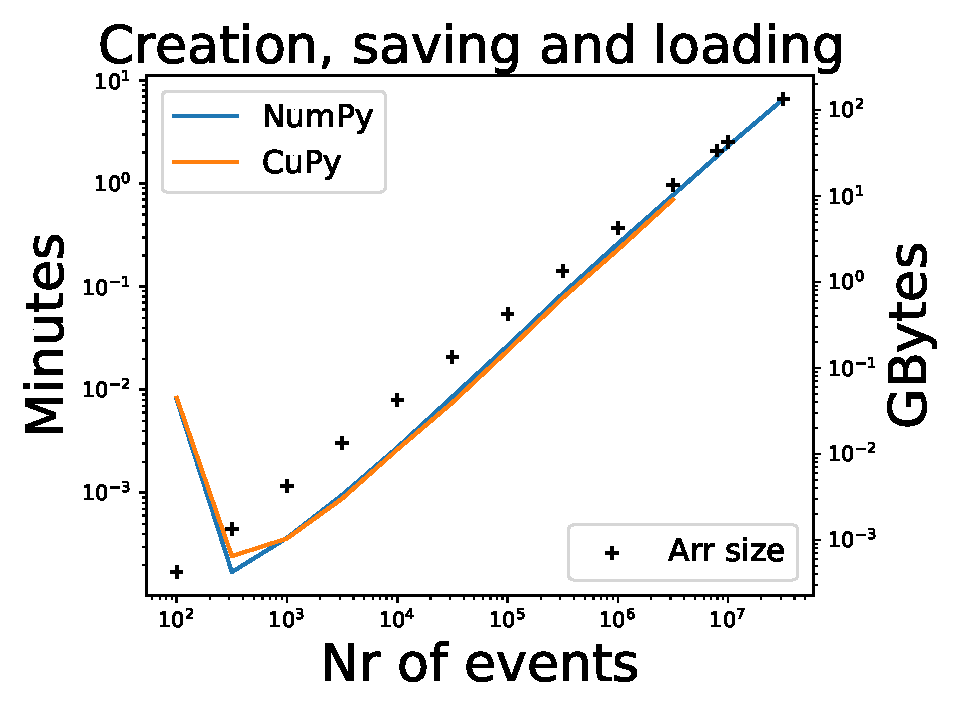
\includegraphics[width=0.7\textwidth]{Figures/atlas/cupy_testing.pdf}
% \end{figure}

% In figure \ref{fig:cupy_comp} we have a comparison in runtime between NumPy and CuPy. The test checks how long time 
% in minutes both libraries take to create a uniformly distributed array of size $Events\times Features$, where the 
% number of features were set to 529, the number of features in the RMM structure used in this thesis. The number of events 
% were set in powers of 10 from 2 to 8, with a half increment, i.e $[2, 2.5, 3, ..., 7.5]$. The GPU used in the test 
% is the same used in the rest of the thesis, an NVIDIA A100-PCIE-40GB. The left y-axis shows the amount of minutes 
% each array took, where the right yaxis shows the array size in Gigabytes. From this figure we really see that this 
% bottleneck is not something one can do much about, unless one can aquire large amounts of GPU memory. An even then, 
% Numpy is still incredibly fast. \par 
Another bottleneck is computation time of training and inference. 
There is a continuing battle between speed and accuracy in terms of choosing an appropriate batchsize. 
The choice of batchsize for this thesis is 8192. It is common to choose a batchsize that is a multiple of two, 
as this is most optimized for GPU's. 8192 is $2^{13}$, and it a rather large batchsize. Allthough this allows for 
epoch training time to be as low as less than 2 minutes for 2 lepton case and less than 1 minute for 3 lepton case,
it does decreace the model's ability to learn more about the dataset\cite{Goodfellow-et-al-2016}. With better and faster equipment this could 
be improved whilst decreasing the batchsize. 


\subsection*{Data and feature engineering}
\subsubsection*{Scaling}
One aspect that was not explored in this thesis is the choice of scaling for the data. The choice used for this 
thesis was the MinMax scaling algorithm from Sci-kit learn. From previous work done on the ATLAS Open data 
\cite{ATL-OREACH-PUB-2020-001} it appeared that MinMax was better for over all accuracy than Standard scaling.
Still, it should be looked at and more understood why this is or is not the case for the Run2 dataset used in this 
thesis. 

\subsubsection*{Interpretation and possible feature changes}
This thesis used the Rapidity-Mass matrix described by Chekanov\cite{Chekanov_2019} as features in the dataset. 
Whilst containing features that are very uncorrelated it creates a feature signature that could be used by 
the autoencoder to learn underlying structures in the SM. There are however some aspects to discuss. 
First, every nonexisting entry in the RMM for a given event is replaced with a zero value. This creates 
"islands" in the RMM structure with contributes to create the signatures for the events. It is however not clear 
how these zero values propagate through the network, and how they affect the performance and really the autoencoder's 
ability to learn the underlying structures in the SM. In cases where one uses tools like decision trees, 
this is not an issue, as they can just remove the feature if it holds a certain value, but as we need a tabular and 
rectangular shape to do the matrix multiplication that is neural network feed forwarding and backpropagation, a value
has to be put in the missing entries, and it is not obvious or known what the choice of using zeros does. \par 
Another choice to consider is the amount of particles in the RMM. This thesis tried allowing for 5 electrons and 5 muons, 
and 6 b- and ljets, yeilding a total of 529 elements in the RMM. This choice was an arbitrary one, but it is not 
unreasonable to think that an even larger RMM would be more beneficial, as it contains more information. Some 
events might have even more jets in them, or leptons. But with a larger RMM comes a larger amount of zero valued 
features as well. And also, with a larger RMM, the memory needed for a given array increases, which in the case of
the 2 lepton case, would mean more megasets of smaller size. The computation time, from event selection and conversion from Rdataframe to Numpy, and training 
and inference, would increase a lot. A third point to make is that the RMM alone might not be the ideal set of features. 
It would be interesting to test a combination of RMM and some other features, were we remove some of the features that are
on average are zero and replace them with other useful information. If the goal is to learn the autoencoders the signature 
of the SM, then it is not unreasonable to assume that more specific information would be better. It should be better understood 
what it means to learn the signature of a channel, and of the SM as a whole. \par 





\subsection*{Architecture engineering}
The regular autoencoder appears to provide a better anomaly detection performance than the variational autoencoder. 
The architecture is somewhat simple, given the hard task it is meant to perform. It might be possible to 
add some more complex layer structures like CNN autoencoders or PCA to make a more complicated and better performing 
network architecture. This is of course only speculation, and was not investigated much in depth. General trends were 
found to vary depending on the size of the dataset, and it is not trivial that for example a deep neural network is 
benefitial as the training sample increases. What was important though was to ensure that the latent space was large 
enough to store enough information for the decoder. In the early attempts the latent space were set between 10 and 50 
nodes, which was too little for the encoded information to be useful. As there is no clear way to find the optimal 
architecture, an educated guess on the number of nodes were done. In theory, one can create a tunable network where 
the number of layers and nodes in each layer are hyperparameters, but the sheer number of combinations would lead to 
much longer computation time than what was available during this thesis. Tools like Keras-Tuner could facilitate 
this search, but if this were a PhD thesis or a long term research project it would be benefitial with more
 significant hardware or a more rigorous way to set an optimal architecture. \par

% Tools like Keras-Tuner could facilitate 
% this search, but one should have significant hardware. Based on the experience from working on this thesis it seems 
% that educated guesses are the best way to find a good architecture, but given the overall search problem it is hard 
% or perhaps no point in doing searches for optimal architectures, more than educated guesses. \par

Another point to think about is how the autoencoder is trained. As explained in section \ref{sec:autoencder_theory}
the autoencoder is trained by how well it manages to reconstruct the input data. This is done by 
calculating the error of each feature for a given event, and averaging the error for all features. 
This has its pros and cons, and should be investigated further. Suppose one has an RMM which is very sparse, 
with 10 bjets, 10 ljets, 10 electrons, 10 muons, and 10 photons, i.e a T5N10 matrix of 2601 colums and rows. 
In this case, one can easily assume that the RMM would be very sparse, as few if any SM events produced 
as the current energy level as the LHC contains that many particles. Thus, one could argue that some features 
are more important to learn correctly than others, and thus should be weighted more. It is however difficult to 
know which features that should be in focus, as the signatures for each event's might differ, and some 
might look completely different from one another. One way to deal with this issue is to calculate 
the average RMM for a given channel, and then see if there are general trends in the RMM for those channels. 
Then one could perhaps weigh the most used features more than the more sparse areas. 